 \documentclass[11pt, oneside]{article}% use "amsart" instead of "article" for AMSLaTeX format
\usepackage[margin = 2.5cm]{geometry}% See geometry.pdf to learn the layout options. There are lots.
\geometry{letterpaper}   % ... or a4paper or a5paper or ... 
\usepackage{graphicx}% Use pdf, png, jpg, or eps§ with pdflatex; use eps in DVI mode
\usepackage{enumitem} 

\usepackage{listings}  %  needed for source code listings
\lstset{language=Java} 
\usepackage[skip=14pt]{caption}
\usepackage{amssymb}
\usepackage{dsfont}
\usepackage[parfill]{}
\usepackage[T1]{fontenc}
\usepackage{titling}
\setlength{\droptitle}{-2.5cm}
\usepackage{setspace}
\usepackage{indentfirst}
\usepackage{float}
\usepackage{wrapfig}
\lstset{frame=lrbt,xleftmargin=\fboxsep,xrightmargin=-\fboxsep}

% set the document title, author, and date here.
%  once set, the \maketitle command (within the document)
%  will display them nicely
\title{Sequence Alignment}
\author{Nicholas Fiacco}

\begin{document}
\maketitle

\section{Introduction}
The world of biological research is rapidly growing thanks to the application of new computational approaches and the different perspectives and insights that can be gathered from previously useless data.  I will be exploring a topic in Bioinformatics (don't tell my research mentor, a professor in the related but distinct field of Computational Biochemistry!), a field that is still relatively young but has already yielded several exciting new discoveries and techniques for analyzing both protein composition and genetic information.  Many of the research efforts in this field seek to gain insights as to the relationships between related molecules by examining their chemical composition and using compositional similarity as a basis for determining structural and functional similarity.  Thus, these techniques are very useful in both drug design and genetics research, since we are able to understand more about an unknown molecule by comparing it to those we have more information about.

In this project, we seek to construct a Hidden Markov Model (HMM) to reason about the similarity of either a strand of DNA or an amino acid chain (protein) to a family of other genes/proteins that are already known to be related.  The method described will not only tell us how similar our query molecule is, but also help us determine the best way to align individual building blocks (nucleotides or amino acids) such that conserved regions are aligned with those of the other sequences in the family.  We will explain how we build the HMM from Multiple Sequence Alignment (MSA) training data from PFAM, and then discuss how to apply this model to the query sequence.  Finally, we will discuss the possibility of constructing the model from unaligned training data using a probabilistic method known as Baum-Welch, and the usefulness of such an approach.

\section{Multiple Sequence Alignment}
First, we will explain the meaning of the underlying sequence used to represent either a protein or strand of DNA, and the motivation for producing an alignment.  A sequence is simply a string of characters that is used to represent the chain of building blocks used to create a macromolecule, with each symbol in the string denoting an amino acid or nucleotide.  A sequence alignment is a way of arranging multiple sequences as rows in a matrix such that regions of similarity are lined up as columns, with dashes (-) inserted to represent gaps between conserved (similar) regions.  Conservation of a region can refer to either the actual compositional similarity, or similarity in terms of the structural importance of that particular region.  Identifying such regions is quite important since a strong correlation might suggest a functional relationship between the sequences under consideration.  Frequently, sequence alignment is performed with more than two sequences at a time, with Multiple Sequence Alignment (MSA) most often applied to a family of related genes or proteins.  This MSA is what we will use as training data for our model, and we can gather such information from the PFAM database (Note: thanks to Professor Grigoryan for pointing me in the direction of PFAM, otherwise I would have had to make my own data and it would not be as interesting).

\newpage


\section{Position-Specific Scoring Matrix}
Based on the MSA, we will need to determine the frequency of each amino acid or nucleotide, henceforth referred to as emissions, specific to each position in the aligned sequences (read: column).  This is a fairly straightforward procedure, and we store the information in a Position-Specific Frequency Matrix (PSFM), which has a column for each position in the MSA and a row for each possible emission.  This PSFM can be used to develop a Position-Specific Scoring Matrix (PSSM), useful in other applications of the MSA for sequence analysis, but not necessary for building our HMM.  Nevertheless, we include a method to construct one since it is fairly trivial given the frequency counts, and will be useful in evaluating the effectiveness of our HMM.
\subsection{Pseudocounts}
Although this method of creating a PSFM is already very effective as described above, it is important to note that any emission that does not occur in our MSA at a particular column will have zero probability of occurring, which does not suit the needs of our emission model which should be general enough to handle any query sequence.  Thus, we initialize our PSFM with a pseudocount of one for each emission at each position, which ensures that we do not overfit the HMM to the MSA which we used to train it.
\subsection{Consensus Sequence}
Every HMM model has a sequence of emissions that is most likely given the transition and emission probabilities.  By applying the Viterbi algorithm to a sequence with the most likely emissions at each position, we can determine the consensus sequence: an alignment of the most likely emissions.  This consensus sequence will also have associated with it a probability for the assignment of a state in the model to each position, and these probabilities represent the upper bound on the likelihood of a given predicted alignment given our model.

\begin{figure}[H]
\centerline{\includegraphics[width=0.5\textwidth]{msa_example}}
  \caption{An example of a MSA, taken from the data used to train the model in this project.  Note, this is a very small piece of that data, and omits some extra information included in a SELEX formatted MSA, which needs to be removed from the MSA before we can construct our PSFM.}
\end{figure}

\newpage


\section{Profile Hidden Markov Model}
\subsection{Overview}
First, we must make the distinction between several related terms.  When developing the model, most of the literature refers to three separate states: match, insert, and delete.  Note that these are not the states we considered when we used a Hidden Markov Model for probabilistic reasoning about the robot localization problem.  Instead, these states are akin to the locations, any of which were possible at a given state in the blind robot problem.  We will consider the group of three states bundled together at a particular time step a node, and it is the nodes that will make up the Hidden Markov Model.  Furthermore, we are not stepping through time, but instead positions in a sequence of amino acids or nucleotides.  Whereas the multiple sequence alignment has inserted gaps to optimize the alignment of the sequences, our query sequence will begin unaligned and it is our job to find the best way to fit the sequence to the model.  We will use the Viterbi algorithm to achieve this, and we will then be able to determine how good of a fit we achieved through a comparison to a consensus sequence.\\

\begin{figure}[H]
\centerline{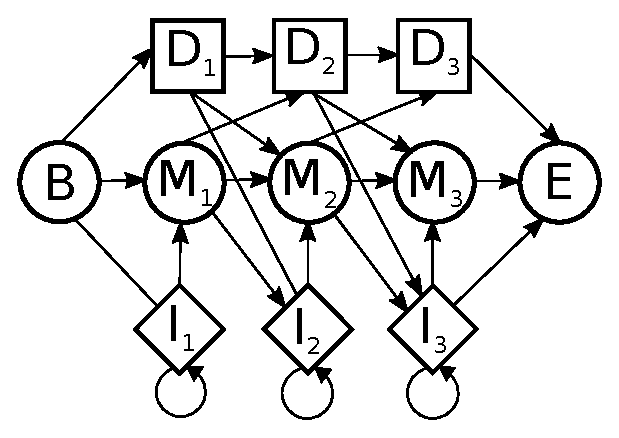
\includegraphics[scale=.8]{hmm}}
  \caption{This is a representation of a Profile Hidden Markov Model with three backbone states.  Note that there is a delete state and insert state corresponding to each match state, and only insert states can transition to another state in the same node.}
\end{figure}

\subsection{Ungapped HMM (Backbone)}
Before we can begin training the model, we must first decide how many nodes are actually represented by the MSA.  This is done by determining which columns in the PSFM are backbone positions: those that are explicitly aligned to demonstrate conserved regions.  However, simply because a single sequence has a gap does not mean that the entire position, or column, is a gap.  We determine backbone states as follows: when more than half of the sequences have an emission at a particular position, this is a backbone position.  Any sequences that emit at this position are in a match state, those that do not are in a delete state.  Thus, delete states are emission-less states, which will be discussed further later on in this report.  Columns in which more than half of the sequences do not emit are not backbone columns, and any sequences that do have emissions in these positions are in insert states.  When a sequence does not emit at a non-backbone column, this is simply an invalid state and is disregarded entirely.  With this distinction made, we can annotated each sequence and construct our transition and emission models.

\subsection{Annotating the Multiple Sequence Alignment}

\begin{figure}[H]
\centerline{\includegraphics[scale=0.7]{backbone}}
  \caption{Here is another example of an MSA, with backbone columns denoted with an asterisk.}
\end{figure}

Once we have determined the backbone columns, we annotate every position in each sequence with one of the three states, which we will use later to determine transitions.  Here is the code for doing just that, called \verb`createAnnotations` and found in \verb`MarkovModel.java`:\\

\begin{lstlisting}
// if this position is a backbone column in the alignment
if(backbone[position]){
  // check whether it is a blank emission
  if(emission != '-'){
    // it is not a blank, so the position is a match
    annotated[seqNum][position] = 0;
  }
  else{
    // it is a blank, so the position is a delete
    annotated[seqNum][position] = 1;
  }
}
else{
  // if the position is not a blank, then it is inset
  // otherwise we can just ignore it
  if(emission != '-'){
    annotated[seqNum][position] = 2;
  }
  else{
    // annotate with -1 to show it is invalid
    annotated[seqNum][position] = -1;
  }
}
\end{lstlisting}   


\section{Building the Optimal Alignment}
\subsection{Viterbi Algorithm}
We use the Viterbi algorithm to find the assignment of states to positions in the query sequence such that the probability is maximized, in other words we find a best path through the states of the model given the emissions of symbols from our query sequence.  Then, given this sequence of states, we can build the aligned sequence by inserting the observed nucleotide at the beginning of a gap when an insert state is assigned, or inserting a space when a delete state is assigned.

The basic concept of the Viterbi algorithm is simple and having an understanding of the forward-backward algorithm, it is easy to describe.  Rather than summing over the probabilities for each state, we simply store the maximum probability associated with transitioning to a particular state, and saving the previous state that incurred this maximum on the optimal path to this state.  It is possible that the most likely path to each state is different, and in practice this is often the case.  However, once we determine the final state with the single highest probability, it is easy to trace back the most likely path if we store every single one, so this is the approach that is used.

The code for finding the most likely path can be found in \verb`MarkovModel.java`, and is called \verb`findBestPath`.  It makes use of methods in both \verb`TransitionModel.java` and \verb`EmissionModel.java`, which are easy to find because they make use of the word Viterbi in their name.  We include in this report the method for constructing the alignment, \verb`constructAlignment`, based on this most likely path, since it is a rather unique aspect of this assignment:\\

\begin{lstlisting}
// loop through the querySequence, extending if you add a gap
int limit = querySequence.length();
for(int i = 0; i < limit; i++){
  if(backbone[i] && index < querySequence.length()){
    if(last && path.get(index).getKey() % 3 == 1){
      aligned.append('-');
      limit++;
      last = false;
    }
    else{
      aligned.append(querySequence.charAt(index));
      last = true;
      index++;
    }
  }
  else{
    if(path.get(index).getKey() % 3 == 2){
      aligned.append(querySequence.charAt(index));
      index++;
    }
    else{
      aligned.append('-');
      limit++;
    }
  }
}
\end{lstlisting}

\subsection{Forward-Backward Smoothing}
Included in the code is a way to run forward-backward smoothing, which turns out to be utterly useless.  By taking a look at the diagram of the HMM above, it is clear that the transitions are strongly one-way.  This means that unlike the robot localization problem, there are several states that are no longer reachable after a certain point.  Thus, the backward part of the algorithm results in several states having zero probability, and rather than smoothing we end up messing everything up.  The forward algorithm by itself is rather effective at determining individual probabilities of a particular state, but this is not as informative since it is the entire sequence we are interested in, and thus Viterbi is the only really effective algorithm to apply in this scenario.

\section{Design and Implementation (IMPORTANT)}
Setting up the model turned out to be the single most difficult part of the project.  Although we had already built a HMM in the probabilistic reasoning assignment, the state transitions and emissions were much more complex in this application, as you can see from the diagram above in Figure 2.  There were several aspects that made this more complicated:
\begin{itemize}
\item Finite model length, unknown query sequence length
\item Emission-less states
\item Self-transitions in certain states
\end{itemize}
We will discuss why each one posed a difficulty in building the model, and discuss the approach taken to resolve each of them.

\subsection{Free Insertion Modules}
Based on the Multiple Sequence Alignment used to train the data, there is a predetermined length to the backbone we use to generate the ungapped HMM, and subsequently there are a fixed number of nodes in the resulting profile Hidden Markov Model.  This raises the question of what will happen when we receive a query that is longer or shorter than the model.  It turns out that when the query sequence is shorter, it will fit the sequence to the best sequential subset of nodes in the model, since we initialize the startVector with pseudocounts for all states allowing the possibility that starting further into the model is more likely.  In the case that the query is longer, we include Free Insertion Modules (FIM) which are special states that have an equal probability of any emission and can only transition to themselves.  By including a FIM at the beginning and end of the module, we allow the model to orient query sequence in the optimal position, despite the fact that the backbone is shorter than the query itself.  Note that the first insert state serves as a FIM that can transition to the match and delete states within the same node.

\subsection{Self-Transitions}
As clearly demonstrated in the diagram in Figure 2, insert states can transition to themselves.  This allows insertions of arbitrary length, but also poses the question of how to handle assigning the same state to multiple positions, albeit with different probabilities.  The logic behind the transitions also took a bit of time to resolve, since the insert nodes should not transition to the next node, but to other states or itself, within the current node.  The code to determine the index of the next states is not too confusing, but lengthy so it will not be included in the report.  It can be found in \verb`TransitionModel.java` within the \verb`viterbiTransition` method.  Another difficulty arises in constructing the alignment from the assignment of states to positions.  That was already demonstrated in the \verb`constructAlignment` method above.

\subsection{Emission-Less States (Most Difficult Part)}
We've already mentioned several times above that handling the delete states was amongst the trickiest parts of this project.  Since these states are emission-less, it does not make sense to pass them into the emission model.  However, when a delete state is highly likely, it means that the emission associated with this position would likely be associated with a match or insert in the next node.  However, these nodes will not be considered because the delete state has not yet transitioned to them at the current iteration through the Viterbi algorithm.  This is a significant problem, and there is absolutely no discussion of the issue in the literature (which makes me very curious how others have handled it).  Thus, the solution I have developed may not be standard, but is quite effective.  Here is a description of what I did:\\

\noindent At the end of each transition step, we loop through the distribution vector again, and propagate the probability of being in any delete states amongst the states it eventually transitions to.  To handle multiple chained deletions, we approach this in node order, so that when a delete state transitions to a future delete state, we are guaranteed to encounter it in a later loop.  This is only possible because of the one-way transitions.  When we reach the end of each loop, we set the probability of each delete state to zero.  Thus, before we apply the emission model to our distribution, we ensure that there is no possibility of being in a delete state.  Essentially, we are doing a half step before moving to the next emission.  The code can be found in \verb`TransitionModel.java` at the method \verb`propagateDelete`, but this description of the process should be sufficient to convey the idea.

\section{Results}
We tested the model by training it first on a short training dataset that I wrote myself, using the symbols "A, T, C, G" to represent nucleotides, and"-" to represent a gap.  With the small dataset, the alignments aren't very informative.  However, with the MSA obtained from the PFAM database, we are able to construct a model of amino-acids sequences that encode the WD40 repeat (I have no idea what that actually is, its just a protein structure).  Here is an example of the input query sequence, the output alignment, and the actual alignment, for comparison:\\

\begin{lstlisting}
Input Sequence: GRCERTFLGHEDCVRGLAILSETEFLSCANDASIRRWQ

Aligned Sequence: GRCERT--F----L-----GH----EDC----------------V---R----
GLA-----------------ILSETEF-----------L---------S--------C---A---N----D
ASIRR--WQ

Actual Alignment: GRCERT--F----L-----GH-----ED------------C---V---R----
GLA-----------------ILSETEF-----------L----S----C--------A---N--------D
ASIRR--WQ
\end{lstlisting}

\noindent It is interesting to examine the example output I have included with my submission with the MSA in selex\_data.txt.

\section{Literature Review}
\centerline{\textit{Generalized Baum-Welch Algorithm Based on the Similarity between Sequences}}
The Baum-Welch algorithm is used for parameter estimation in the absence of a Multiple Sequence Alignment from which we can determine probabilities for each emission and transition.  Whereas for the robot localization problem we were given the probabilities for the sensor readings and could easily compute transition probabilities, this is not the case with the sequence alignment problem.  Similarly, if we are given a multiple sequence alignment, then it is easy to build a PSSM since the $i^{th}$ position in each sequence is aligned with that of the others.  We can then determine which columns to include in our backbone and build our HMM parameters based on this information.  However, when we are provided unaligned data, this process is no longer possible.  Instead, we can use an algorithm known as Baum-Welch which employs iterative processing of sequences using the forward algorithm to estimate probabilities for each state, each time using the final distribution as the parameters for the HMM on the next sequence.

This paper, by Rezaei et. Al, discusses a method for enhancing the Baum-Welch algorithm by using known substitution probabilities for amino acids in the construction of the emission model.  Basically what this means is that all of the amino acids have specific properties which make them unique, and some have more in common than others (for example being hydrophilic or hydrophobic).  Thus, there is a higher probability associated with emitting certain amino acids even if they have never been seen before.  Essentially, they modified the pseudocounts to reflect these substitution probabilities once the PSFM was created.  I would like to point out that their model omits certain transitions that I included in my implementation, such as Delete $\rightarrow$ Insert.

\subsection{References}

\noindent Baldi.P., Chauvin.Y., Hunkapillar.T. and McClure,M. "Hidden Markov models of biological primary sequence information." (1994). Proc. Natl Acad. Set. USA, 91, 1059-1063.\\

\noindent S R Eddy "Profile hidden Markov models". (1998). Bioinformatics.\\

\noindent Krogh, A. "An introduction to hidden Markov models for biological sequences." (1998). In Salzberg, S.; Searls, D.; and Kasif, S., eds., Computational Methods in Molecular Biology. Elsevier.\\

\noindent Mimouni, Naila, Gerton Lunter, and Charlotte Deane. "Hidden Markov Models for Protein Sequence Alignment." (2005). University of Oxford. Print.\\

\noindent Rezaei V, Pezeshk H, P�rez-Sanchez H "Generalized Baum-Welch algorithm based on the similarity between sequences." (2013). PLoS One.\\

\noindent Robert D. Finn, Penelope Coggill, Ruth Y. Eberhardt, Sean R. Eddy, Jaina Mistry, Alex L. Mitchell, Simon C. Potter, Marco Punta, Matloob Qureshi, Amaia Sangrador-Vegas, Gustavo A. Salazar, John Tate, and Alex Bateman "The Pfam protein families database: towards a more sustainable future." (2016). Nucl. Acids Res.\\

\noindent Yoon, Byung-Jun. "Hidden Markov Models and Their Applications in Biological Sequence Analysis." Current Genomics 10.6 (2009): 402-415. PMC.\\



\end{document}





























